Salah satu tujuan utama penelitian ini adalah mengatasi keterbatasan LiDAR 2D dalam mendeteksi obstacle yang berada di luar bidang pindai horizontal sensor. Sebagaimana dijelaskan pada Bab~I dan Bab~III, LiDAR 2D hanya melakukan pengukuran pada satu bidang datar sehingga obstacle yang memiliki tinggi lebih rendah dari bidang pemindaian berpotensi tidak terdeteksi meskipun secara fisik berada pada jalur pergerakan robot (\cite{Fagundes2024,Kibii2022}). Kondisi tersebut dikenal sebagai \textit{blind-spot} vertikal dan menjadi salah satu penyebab utama terjadinya kolisi pada sistem navigasi yang hanya mengandalkan sensor LiDAR 2D.

Untuk mengevaluasi kemampuan sistem dalam mengatasi permasalahan tersebut, pada penelitian ini digunakan obstacle berprofil rendah berupa model kucing yang ditempatkan pada jalur navigasi robot. Obstacle tersebut dirancang agar sebagian besar berada di luar bidang observasi LiDAR sehingga tidak dapat direpresentasikan secara memadai pada data \textit{LaserScan}. Sebaliknya, obstacle masih dapat diamati oleh kamera termal sehingga informasi keberadaannya dapat dimanfaatkan dalam proses pembentukan traversability termal dan \textit{virtual scan}.

\subsection{Perbandingan Kejadian Tabrakan pada Obstacle Blind-Spot}

Jumlah kejadian tabrakan terhadap obstacle kucing pada seluruh skenario yang mengandung area \textit{blind-spot} ditunjukkan pada Gambar~\ref{fig:cat_collision}.

\begin{figure}[H]
\centering
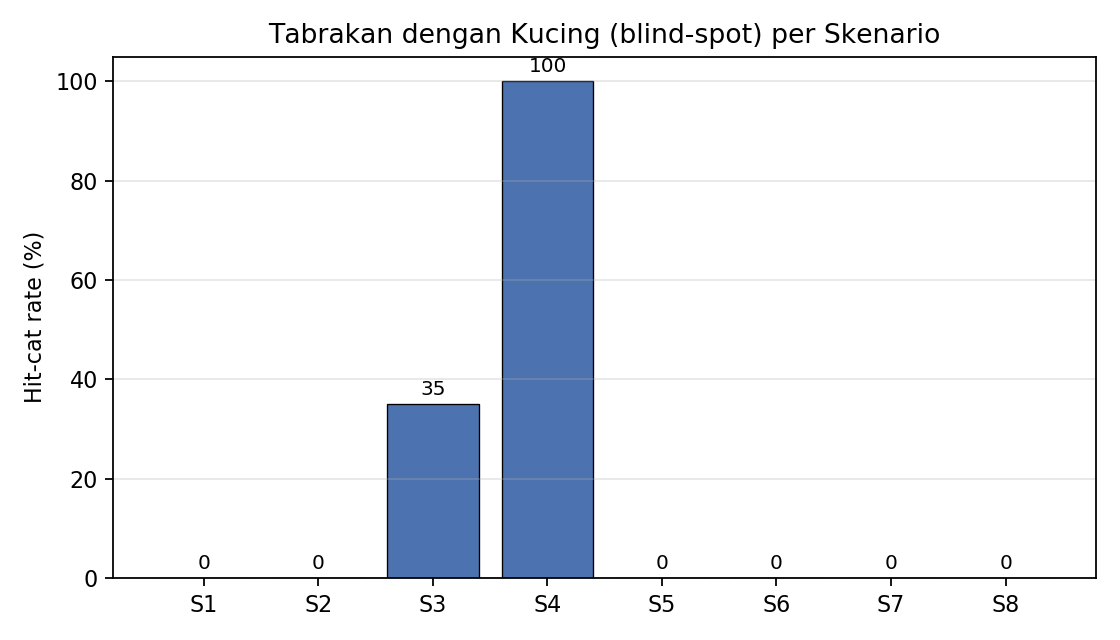
\includegraphics[width=0.75\textwidth]{gambar/fig_hit_cat.png}
\caption{Jumlah kejadian tabrakan terhadap obstacle berprofil rendah pada area blind-spot LiDAR.}
\label{fig:cat_collision}
\end{figure}

Hasil pengujian menunjukkan bahwa konfigurasi baseline mengalami kegagalan yang leb\-ih sering ketika berhadapan dengan obstacle berprofil rendah. Pada konfigurasi ini, sebagian obstacle tidak terdeteksi secara memadai oleh LiDAR sehingga robot tetap bergerak menuju tujuan tanpa melakukan manuver penghindaran yang cukup.

Sebaliknya, konfigurasi fuzzy yang memanfaatkan integrasi kamera termal menunjukkan penurunan jumlah kejadian tabrakan yang sangat signifikan. Informasi termal yang diperoleh dari kamera memungkinkan sistem mengenali keberadaan obstacle meskipun obstacle tersebut berada di luar bidang pemindaian LiDAR. Informasi tersebut kemudian diproyeksikan ke dalam representasi navigasi melalui proses pembentukan \textit{virtual scan} dan perhitungan traversability sehingga obstacle dapat diperhitungkan oleh planner lokal selama proses navigasi.

Temuan ini konsisten dengan hasil pada Subbab~4.3 dan Subbab~4.4 yang menunjukkan peningkatan \textit{Success Rate}, \textit{Collision-Free Rate}, dan \textit{minimum clearance} pada konfigurasi fuzzy. Dengan kata lain, peningkatan performa yang diamati tidak hanya berasal dari perubahan strate\-gi navigasi, tetapi juga dari peningkatan kualitas persepsi lingkungan yang diperoleh melalui integrasi kamera termal.

\subsection{Kontribusi Kamera Termal terhadap Persepsi Lingkungan}

Keunggulan utama kamera termal pada penelitian ini terletak pada kemampuannya menyediakan informasi tambahan pada area yang tidak dapat diamati secara optimal oleh LiDAR 2D. Ketika obstacle berada di luar bidang pemindaian laser, data LiDAR tidak lagi cukup untuk merepresentasikan kondisi lingkungan secara lengkap. Pada kondisi tersebut, kamera termal berperan sebagai sensor komplementer yang menyediakan informasi keberadaan obstacle berdasarkan karakteristik termalnya.

Berbeda dengan pendekatan yang hanya menggunakan kamera sebagai sensor deteksi objek, penelitian ini memanfaatkan informasi termal untuk membentuk estimasi traversability lingkungan yang kemudian digabungkan dengan traversability berbasis LiDAR melalui meka\-nisme fusi sensor. Pendekatan tersebut memungkinkan sistem menghasilkan representasi lingk\-ungan yang lebih lengkap tanpa mengubah struktur dasar ROS Navigation Stack yang digunakan.

Hasil eksperimen menunjukkan bahwa kombinasi antara traversability LiDAR, traversability termal, dan pengendali fuzzy menghasilkan peningkatan kemampuan navigasi terutama pada kondisi yang sebelumnya menjadi kelemahan utama LiDAR 2D. Dengan demikian, kamera termal tidak hanya berfungsi sebagai sensor tambahan, tetapi berperan langsung dalam meningkatkan keselamatan navigasi melalui pengurangan risiko tabrakan terhadap obstacle pada area \textit{blind-spot}.

\subsection{Implikasi terhadap Tujuan Penelitian}

Berdasarkan seluruh hasil pengujian yang telah dipaparkan pada Subbab~4.3 hingga Subbab~4.7, dapat disimpulkan bahwa metode yang diusulkan berhasil mengatasi sebagian keterbatasan persepsi yang dimiliki LiDAR 2D pada lingkungan indoor. Integrasi kamera termal memungkinkan obstacle berprofil rendah tetap terdeteksi meskipun tidak berada pada bidang pemindaian laser, sedangkan mekanisme fuzzy membantu robot merespons kondisi tersebut secara adaptif melalui penyesuaian parameter navigasi.

Temuan ini mendukung hipotesis bahwa fusi sensor LiDAR dan kamera termal mampu meningkatkan keselamatan navigasi robot bergerak pada lingkungan yang mengandung obstacle berprofil rendah. Selain meningkatkan \textit{minimum clearance}, metode yang diusulkan juga mempertahankan tingkat keberhasilan navigasi yang tinggi serta mengurangi kejadian tabrakan pada area yang sebelumnya menjadi \textit{blind-spot} bagi LiDAR 2D.
